\resizebox{0.98\columnwidth}{!}{
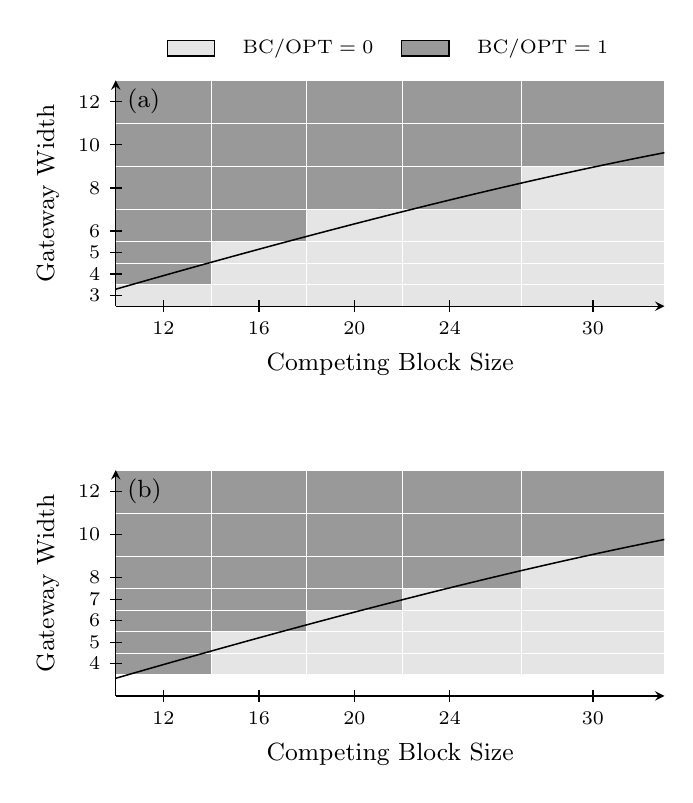
\begin{tikzpicture}
\begin{axis}[
width=8.55cm,height=4.45cm,
at={(0,4.95cm)},anchor=south west,
axis lines=left,axis on top,
axis line style={black,line width=0.5pt},
tick style={black,line width=0.45pt},
tick label style={font=\scriptsize},label style={font=\small},
xmin=10,xmax=33,ymin=2.5,ymax=13,
xtick={12,16,20,24,30},
ytick={3,4,5,6,8,10,12},
xlabel={Competing Block Size},ylabel={Gateway Width},
legend style={draw=none,fill=none,font=\scriptsize,legend columns=2,at={(0.5,1.05)},anchor=south,column sep=8pt},
clip=true
]
\path[fill=black!10,draw=white,line width=0.25pt] (axis cs:10,2.5) rectangle (axis cs:14,3.5);
\path[fill=black!40,draw=white,line width=0.25pt] (axis cs:10,3.5) rectangle (axis cs:14,4.5);
\path[fill=black!40,draw=white,line width=0.25pt] (axis cs:10,4.5) rectangle (axis cs:14,5.5);
\path[fill=black!40,draw=white,line width=0.25pt] (axis cs:10,5.5) rectangle (axis cs:14,7);
\path[fill=black!40,draw=white,line width=0.25pt] (axis cs:10,7) rectangle (axis cs:14,9);
\path[fill=black!40,draw=white,line width=0.25pt] (axis cs:10,9) rectangle (axis cs:14,11);
\path[fill=black!40,draw=white,line width=0.25pt] (axis cs:10,11) rectangle (axis cs:14,13);
\path[fill=black!10,draw=white,line width=0.25pt] (axis cs:14,2.5) rectangle (axis cs:18,3.5);
\path[fill=black!10,draw=white,line width=0.25pt] (axis cs:14,3.5) rectangle (axis cs:18,4.5);
\path[fill=black!10,draw=white,line width=0.25pt] (axis cs:14,4.5) rectangle (axis cs:18,5.5);
\path[fill=black!40,draw=white,line width=0.25pt] (axis cs:14,5.5) rectangle (axis cs:18,7);
\path[fill=black!40,draw=white,line width=0.25pt] (axis cs:14,7) rectangle (axis cs:18,9);
\path[fill=black!40,draw=white,line width=0.25pt] (axis cs:14,9) rectangle (axis cs:18,11);
\path[fill=black!40,draw=white,line width=0.25pt] (axis cs:14,11) rectangle (axis cs:18,13);
\path[fill=black!10,draw=white,line width=0.25pt] (axis cs:18,2.5) rectangle (axis cs:22,3.5);
\path[fill=black!10,draw=white,line width=0.25pt] (axis cs:18,3.5) rectangle (axis cs:22,4.5);
\path[fill=black!10,draw=white,line width=0.25pt] (axis cs:18,4.5) rectangle (axis cs:22,5.5);
\path[fill=black!10,draw=white,line width=0.25pt] (axis cs:18,5.5) rectangle (axis cs:22,7);
\path[fill=black!40,draw=white,line width=0.25pt] (axis cs:18,7) rectangle (axis cs:22,9);
\path[fill=black!40,draw=white,line width=0.25pt] (axis cs:18,9) rectangle (axis cs:22,11);
\path[fill=black!40,draw=white,line width=0.25pt] (axis cs:18,11) rectangle (axis cs:22,13);
\path[fill=black!10,draw=white,line width=0.25pt] (axis cs:22,2.5) rectangle (axis cs:27,3.5);
\path[fill=black!10,draw=white,line width=0.25pt] (axis cs:22,3.5) rectangle (axis cs:27,4.5);
\path[fill=black!10,draw=white,line width=0.25pt] (axis cs:22,4.5) rectangle (axis cs:27,5.5);
\path[fill=black!10,draw=white,line width=0.25pt] (axis cs:22,5.5) rectangle (axis cs:27,7);
\path[fill=black!40,draw=white,line width=0.25pt] (axis cs:22,7) rectangle (axis cs:27,9);
\path[fill=black!40,draw=white,line width=0.25pt] (axis cs:22,9) rectangle (axis cs:27,11);
\path[fill=black!40,draw=white,line width=0.25pt] (axis cs:22,11) rectangle (axis cs:27,13);
\path[fill=black!10,draw=white,line width=0.25pt] (axis cs:27,2.5) rectangle (axis cs:33,3.5);
\path[fill=black!10,draw=white,line width=0.25pt] (axis cs:27,3.5) rectangle (axis cs:33,4.5);
\path[fill=black!10,draw=white,line width=0.25pt] (axis cs:27,4.5) rectangle (axis cs:33,5.5);
\path[fill=black!10,draw=white,line width=0.25pt] (axis cs:27,5.5) rectangle (axis cs:33,7);
\path[fill=black!10,draw=white,line width=0.25pt] (axis cs:27,7) rectangle (axis cs:33,9);
\path[fill=black!40,draw=white,line width=0.25pt] (axis cs:27,9) rectangle (axis cs:33,11);
\path[fill=black!40,draw=white,line width=0.25pt] (axis cs:27,11) rectangle (axis cs:33,13);
\addplot[black,line width=0.55pt,mark=none,domain=10:33,samples=201,forget plot] {(-(2*(60-x)-2)+sqrt((2*(60-x)-2)^2+8*2*(60-x)*x/6))/2};
\addlegendimage{area legend,draw=none,fill=black!10}
\addlegendentry{$\mathrm{BC}/\mathrm{OPT}=0$}
\addlegendimage{area legend,draw=none,fill=black!40}
\addlegendentry{$\mathrm{BC}/\mathrm{OPT}=1$}
\node[anchor=north west,font=\small,inner sep=2pt] at (rel axis cs:0.01,0.99) {(a)};
\end{axis}
\begin{axis}[
width=8.55cm,height=4.45cm,
at={(0,0)},anchor=south west,
axis lines=left,axis on top,
axis line style={black,line width=0.5pt},
tick style={black,line width=0.45pt},
tick label style={font=\scriptsize},label style={font=\small},
xmin=10,xmax=33,ymin=2.5,ymax=13,
xtick={12,16,20,24,30},
ytick={4,5,6,7,8,10,12},
xlabel={Competing Block Size},ylabel={Gateway Width},
legend style={draw=none,fill=none,font=\scriptsize,legend columns=2,at={(0.5,1.05)},anchor=south,column sep=8pt},
clip=true
]
\path[fill=black!40,draw=white,line width=0.25pt] (axis cs:10,3.5) rectangle (axis cs:14,4.5);
\path[fill=black!40,draw=white,line width=0.25pt] (axis cs:10,4.5) rectangle (axis cs:14,5.5);
\path[fill=black!40,draw=white,line width=0.25pt] (axis cs:10,5.5) rectangle (axis cs:14,6.5);
\path[fill=black!40,draw=white,line width=0.25pt] (axis cs:10,6.5) rectangle (axis cs:14,7.5);
\path[fill=black!40,draw=white,line width=0.25pt] (axis cs:10,7.5) rectangle (axis cs:14,9);
\path[fill=black!40,draw=white,line width=0.25pt] (axis cs:10,9) rectangle (axis cs:14,11);
\path[fill=black!40,draw=white,line width=0.25pt] (axis cs:10,11) rectangle (axis cs:14,13);
\path[fill=black!10,draw=white,line width=0.25pt] (axis cs:14,3.5) rectangle (axis cs:18,4.5);
\path[fill=black!10,draw=white,line width=0.25pt] (axis cs:14,4.5) rectangle (axis cs:18,5.5);
\path[fill=black!40,draw=white,line width=0.25pt] (axis cs:14,5.5) rectangle (axis cs:18,6.5);
\path[fill=black!40,draw=white,line width=0.25pt] (axis cs:14,6.5) rectangle (axis cs:18,7.5);
\path[fill=black!40,draw=white,line width=0.25pt] (axis cs:14,7.5) rectangle (axis cs:18,9);
\path[fill=black!40,draw=white,line width=0.25pt] (axis cs:14,9) rectangle (axis cs:18,11);
\path[fill=black!40,draw=white,line width=0.25pt] (axis cs:14,11) rectangle (axis cs:18,13);
\path[fill=black!10,draw=white,line width=0.25pt] (axis cs:18,3.5) rectangle (axis cs:22,4.5);
\path[fill=black!10,draw=white,line width=0.25pt] (axis cs:18,4.5) rectangle (axis cs:22,5.5);
\path[fill=black!10,draw=white,line width=0.25pt] (axis cs:18,5.5) rectangle (axis cs:22,6.5);
\path[fill=black!40,draw=white,line width=0.25pt] (axis cs:18,6.5) rectangle (axis cs:22,7.5);
\path[fill=black!40,draw=white,line width=0.25pt] (axis cs:18,7.5) rectangle (axis cs:22,9);
\path[fill=black!40,draw=white,line width=0.25pt] (axis cs:18,9) rectangle (axis cs:22,11);
\path[fill=black!40,draw=white,line width=0.25pt] (axis cs:18,11) rectangle (axis cs:22,13);
\path[fill=black!10,draw=white,line width=0.25pt] (axis cs:22,3.5) rectangle (axis cs:27,4.5);
\path[fill=black!10,draw=white,line width=0.25pt] (axis cs:22,4.5) rectangle (axis cs:27,5.5);
\path[fill=black!10,draw=white,line width=0.25pt] (axis cs:22,5.5) rectangle (axis cs:27,6.5);
\path[fill=black!10,draw=white,line width=0.25pt] (axis cs:22,6.5) rectangle (axis cs:27,7.5);
\path[fill=black!40,draw=white,line width=0.25pt] (axis cs:22,7.5) rectangle (axis cs:27,9);
\path[fill=black!40,draw=white,line width=0.25pt] (axis cs:22,9) rectangle (axis cs:27,11);
\path[fill=black!40,draw=white,line width=0.25pt] (axis cs:22,11) rectangle (axis cs:27,13);
\path[fill=black!10,draw=white,line width=0.25pt] (axis cs:27,3.5) rectangle (axis cs:33,4.5);
\path[fill=black!10,draw=white,line width=0.25pt] (axis cs:27,4.5) rectangle (axis cs:33,5.5);
\path[fill=black!10,draw=white,line width=0.25pt] (axis cs:27,5.5) rectangle (axis cs:33,6.5);
\path[fill=black!10,draw=white,line width=0.25pt] (axis cs:27,6.5) rectangle (axis cs:33,7.5);
\path[fill=black!10,draw=white,line width=0.25pt] (axis cs:27,7.5) rectangle (axis cs:33,9);
\path[fill=black!40,draw=white,line width=0.25pt] (axis cs:27,9) rectangle (axis cs:33,11);
\path[fill=black!40,draw=white,line width=0.25pt] (axis cs:27,11) rectangle (axis cs:33,13);
\addplot[black,line width=0.55pt,mark=none,domain=10:33,samples=201,forget plot] {(-(2*(60-x)-3)+sqrt((2*(60-x)-3)^2+8*3*(60-x)*x/9))/2};
\node[anchor=north west,font=\small,inner sep=2pt] at (rel axis cs:0.01,0.99) {(b)};
\end{axis}
\end{tikzpicture}
}
